\begin{figure}[H]
    \centering
    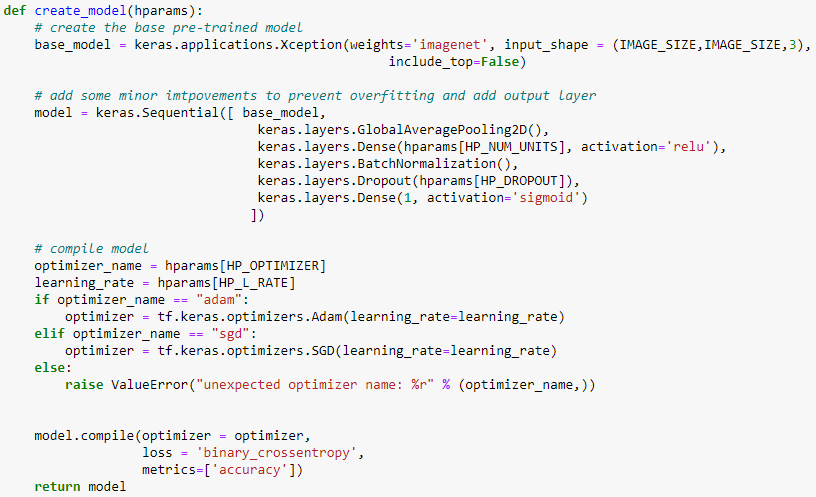
\includegraphics[width=\textwidth]{figures/xception-model.png}
    \caption{The Xception model.}
    \label{fig:xception-model-final}
\end{figure}
\begin{figure}[H]
    \centering
    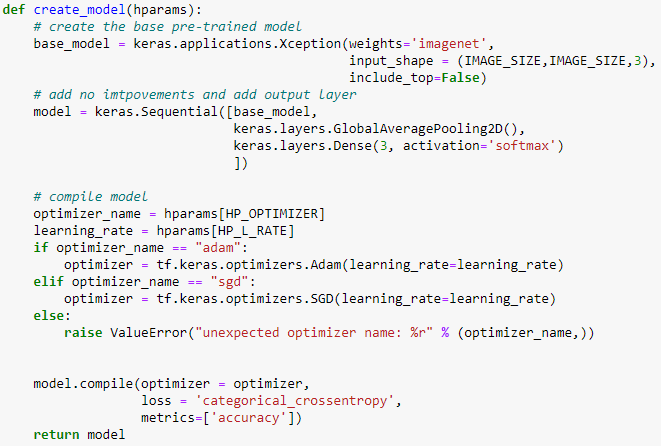
\includegraphics[width=\textwidth]{figures/xception-model-no-improv.png}
    \caption{The Xception model with no improvements.}
    \label{fig:xception-model-final-no-improv}
\end{figure}
\begin{figure}[H]
    \centering
    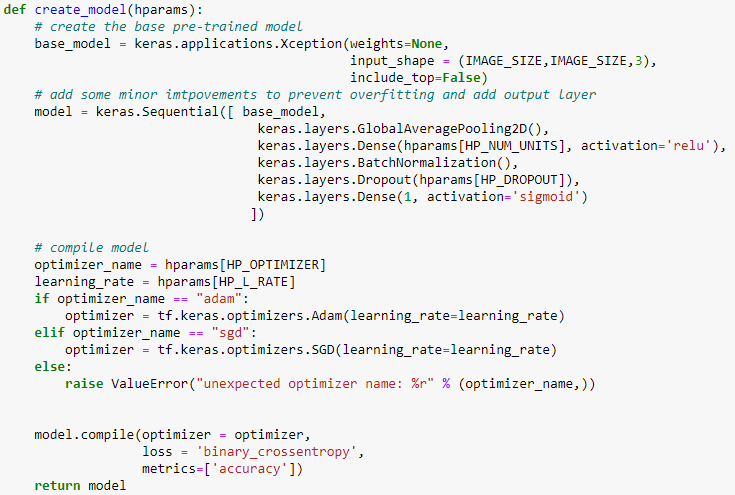
\includegraphics[width=\textwidth]{figures/xception-model-no-weights.png}
    \caption{The Xception model with no pre-trained weights.}
    \label{fig:xception-model-final-no-weights}
\end{figure}
\begin{landscape}
\begin{table}
\caption{Final training results of the binary classification performance of the Xception models, with improvements from this study, without improvements and without pre-trained weights}
\centering
    \begin{tabular}{l|l|l|l|l|l|l|l}
    Model & \begin{tabular}[c]{@{}l@{}}Mean Validation\\ Accuracy\end{tabular} & \begin{tabular}[c]{@{}l@{}}Mean Test\\  Accuracy\end{tabular} & \begin{tabular}[c]{@{}l@{}}Best Fold\\ Test Accuracy\end{tabular} & \begin{tabular}[c]{@{}l@{}}Mean Test\\ Precision\end{tabular} & \begin{tabular}[c]{@{}l@{}}Mean Test\\ Recall\end{tabular} & \begin{tabular}[c]{@{}l@{}}Mean Test\\ F1 Score\end{tabular} & \begin{tabular}[c]{@{}l@{}}Mean Training \\ Time (s)\end{tabular} \\ \hline\hline
    \multicolumn{8}{c}{SMALL DATASET} \\ \hline
    \begin{tabular}[c]{@{}l@{}}Xception\\ \textit{Original improvements}\end{tabular} & 0.9673 & 0.9780 & 0.9950 & 0.9919 & 0.9640 & 0.9775 & 1203 \\
    \begin{tabular}[c]{@{}l@{}}Xception\\ \textit{No improvements}\end{tabular} & 0.9707 & 0.9730 & 0.9925 & 0.9829 & 0.9630 & 0.9725 & 795 \\
    \begin{tabular}[c]{@{}l@{}}Xception\\ \textit{No weights}\end{tabular} & 0.5000 & 0.5000 & 0.5000 & 0.4000 & 0.8000 & 0.5333 & 227 \\ \hline
    \multicolumn{8}{c}{LARGE DATASET} \\ \hline
    \begin{tabular}[c]{@{}l@{}}Xception\\ \textit{Original improvements}\end{tabular} & 0.9630 & 0.9670 & 0.9875 & 0.9632 & 0.9720 & 0.9671 & 7413 \\
    \begin{tabular}[c]{@{}l@{}}Xception\\ \textit{No improvements}\end{tabular} & 0.9733 & 0.9380 & 0.9900 & 0.9901 & 0.8860 & 0.9281 & 7212 \\
    \begin{tabular}[c]{@{}l@{}}Xception \\ \textit{No weights}\end{tabular} & 0.9459 & 0.9625 & 0.9875 & 0.9741 & 0.9520 & 0.9621 & 9893
    \end{tabular}
    \label{fig:xception-model-final-results}
\end{table}
\end{landscape}
\begin{landscape}
\begin{table}
\centering
\caption{Final training results of the multi-label classification performance of the Xception models, with improvements from this study, and without.}
    \begin{tabular}{l|l|l|l|l|l|l|l}
    Model & \begin{tabular}[c]{@{}l@{}}Mean Validation\\ Accuracy\end{tabular} & \begin{tabular}[c]{@{}l@{}}Mean Test\\ Accuracy\end{tabular} & \begin{tabular}[c]{@{}l@{}}Best Fold\\ Test Accuracy\end{tabular} & \begin{tabular}[c]{@{}l@{}}Mean Test\\ Precision\end{tabular} & \begin{tabular}[c]{@{}l@{}}Mean Test\\ Recall\end{tabular} & \begin{tabular}[c]{@{}l@{}}Mean Test\\ F1 Score\end{tabular} & \begin{tabular}[c]{@{}l@{}}Mean Training \\ Time (s)\end{tabular} \\ \hline\hline
    \multicolumn{8}{c}{SMALL   DATASET} \\ \hline
    \begin{tabular}[c]{@{}l@{}}Xception\\ \textit{No Improvements}\end{tabular} & 0.8507 & 0.8110 & 0.9600 & 0.8461 & 0.8450 & 0.8018 & 545 \\
    \begin{tabular}[c]{@{}l@{}}Xception\\ \textit{Original Improvements}\end{tabular} & 0.9274 & 0.9335 & 0.9525 & 0.9185 & 0.9267 & 0.9219 & 673 \\ \hline
    \multicolumn{8}{c}{LARGE DATASET} \\ \hline
    \begin{tabular}[c]{@{}l@{}}Xception\\ \textit{No Improvements}\end{tabular} & 0.9395 & 0.9565 & 0.9700 & 0.9499 & 0.9453 & 0.9468 & 7804 \\
    \begin{tabular}[c]{@{}l@{}}Xception\\ \textit{Original Improvements}\end{tabular} & 0.9466 & 0.9530 & 0.9725 & 0.9436 & 0.9460 & 0.9441 & 7973
    \end{tabular}
    \label{fig:xception-model-multi-results}
\end{table}
\end{landscape}

\begin{figure}
    \centering
    \begin{subfigure}[b]{0.49\textwidth}
        \centering
        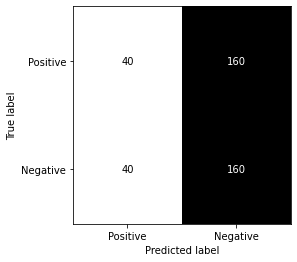
\includegraphics[width=\textwidth]{figures/cm-n-weight-s-b.png}
        \caption{Small binary dataset.}
        \label{fig:cm-n-weight-s-b}
    \end{subfigure}
    \hfill
    \begin{subfigure}[b]{0.49\textwidth}
        \centering
        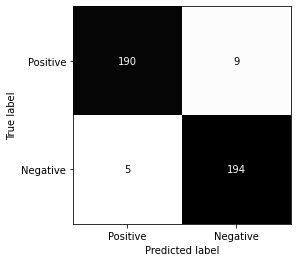
\includegraphics[width=\textwidth]{figures/cm-n-weight-l-b.png}
        \caption{Large binary dataset.}
        \label{fig:cm-n-weight-l-b}
    \end{subfigure}
    \caption{Confusion matrices for the Xception without weights.}
    \label{fig:cm-no-weights}
\end{figure}

\begin{figure}
    \centering
    \begin{subfigure}[b]{0.49\textwidth}
        \centering
        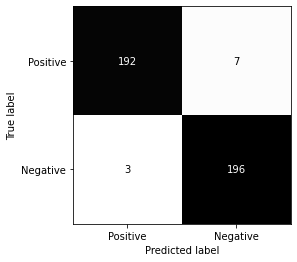
\includegraphics[width=\textwidth]{figures/cm-no-improv-s-b.png}
        \caption{Small binary dataset.}
        \label{fig:cm-n-improv-s-b}
    \end{subfigure}
    \hfill
    \begin{subfigure}[b]{0.49\textwidth}
        \centering
        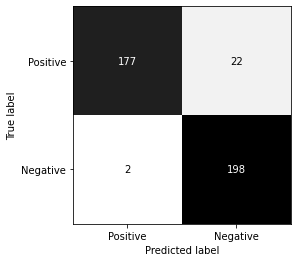
\includegraphics[width=\textwidth]{figures/cm-no-improv-l-b.png}
        \caption{Large binary dataset.}
        \label{fig:cm-n-improv-l-b}
    \end{subfigure}
    \vspace{10mm} %10mm vertical space
    
    \begin{subfigure}[b]{0.49\textwidth}
        \centering
        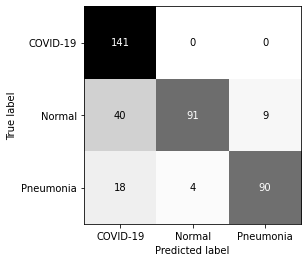
\includegraphics[width=\textwidth]{figures/cm-no-improv-s-m.png}
        \caption{Small multi-label dataset.}
        \label{fig:cm-n-improv-s-m}
    \end{subfigure}
    \hfill
    \begin{subfigure}[b]{0.49\textwidth}
        \centering
        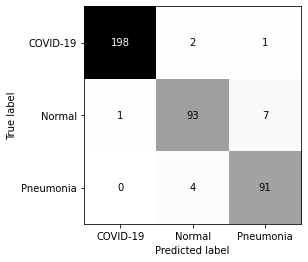
\includegraphics[width=\textwidth]{figures/cm-no-improv-l-m.png}
        \caption{Large multi-label dataset.}
        \label{fig:cm-n-improv-l-m}
    \end{subfigure}
    \caption{Confusion matrices for the Xception without improvements.}
    \label{fig:cm-no-improv}
\end{figure}

\begin{figure}
    \centering
    \begin{subfigure}[b]{0.49\textwidth}
        \centering
        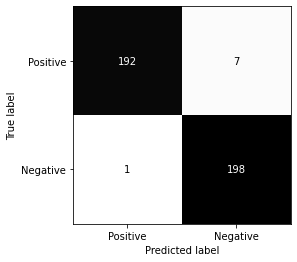
\includegraphics[width=\textwidth]{figures/cm-orig-s-b.png}
        \caption{Small binary dataset.}
        \label{fig:cm-orig-s-b}
    \end{subfigure}
    \hfill
    \begin{subfigure}[b]{0.49\textwidth}
        \centering
        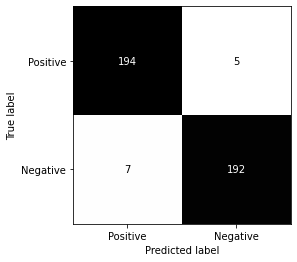
\includegraphics[width=\textwidth]{figures/cm-orig-l-b.png}
        \caption{Large binary dataset.}
        \label{fig:cm-orig-l-b}
    \end{subfigure}
    \vspace{10mm} %10mm vertical space
    
    \begin{subfigure}[b]{0.49\textwidth}
        \centering
        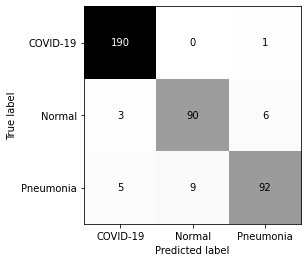
\includegraphics[width=\textwidth]{figures/cm-orig-s-m.png}
        \caption{Small multi-label dataset.}
        \label{fig:cm-orig-s-m}
    \end{subfigure}
    \hfill
    \begin{subfigure}[b]{0.49\textwidth}
        \centering
        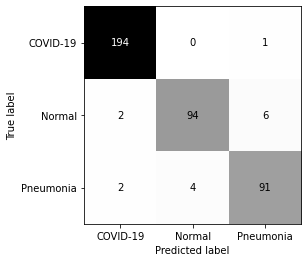
\includegraphics[width=\textwidth]{figures/cm-orig-l-m.png}
        \caption{Large multi-label dataset.}
        \label{fig:cm-orig-l-m}
    \end{subfigure}
    \caption{Confusion matrices for the final XceptionCov19 model.}
    \label{fig:cm-orig}
\end{figure}

\begin{figure}
     \centering
     \begin{subfigure}[b]{0.49\textwidth}
         \centering
         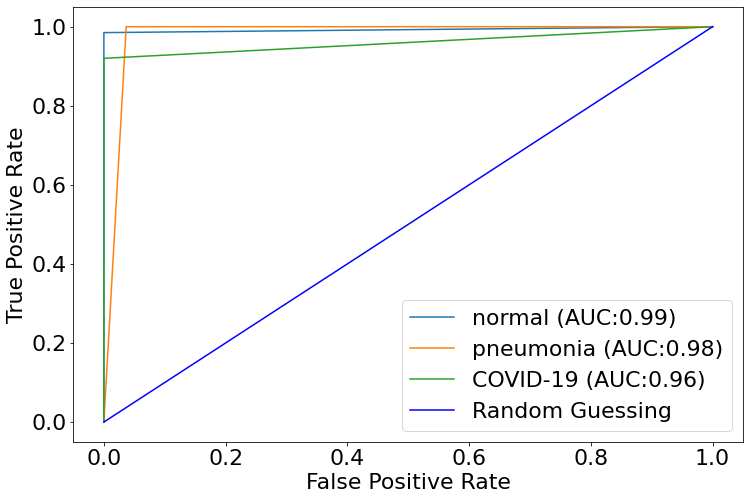
\includegraphics[width=\textwidth]{figures/au-roc-1.png}
         \caption{Fold 1}
         \label{fig:auroc-fold-1}
     \end{subfigure}
     \hfill
     \begin{subfigure}[b]{0.49\textwidth}
         \centering
         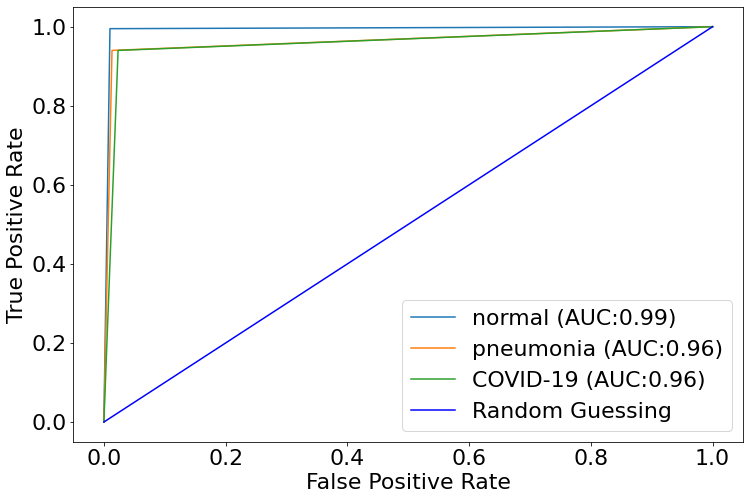
\includegraphics[width=\textwidth]{figures/au-roc-2.png}
         \caption{Fold 2}
         \label{fig:auroc-fold-2}
     \end{subfigure}
     
     \vspace{10mm} %10mm vertical space
     \begin{subfigure}[b]{0.49\textwidth}
         \centering
         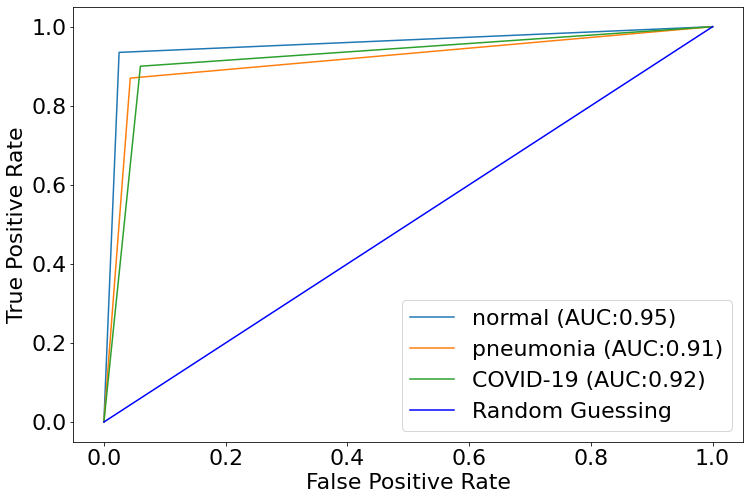
\includegraphics[width=\textwidth]{figures/au-roc-3.png}
         \caption{Fold 3}
         \label{fig:auroc-fold-3}
     \end{subfigure}
     \hfill
     \begin{subfigure}[b]{0.49\textwidth}
         \centering
         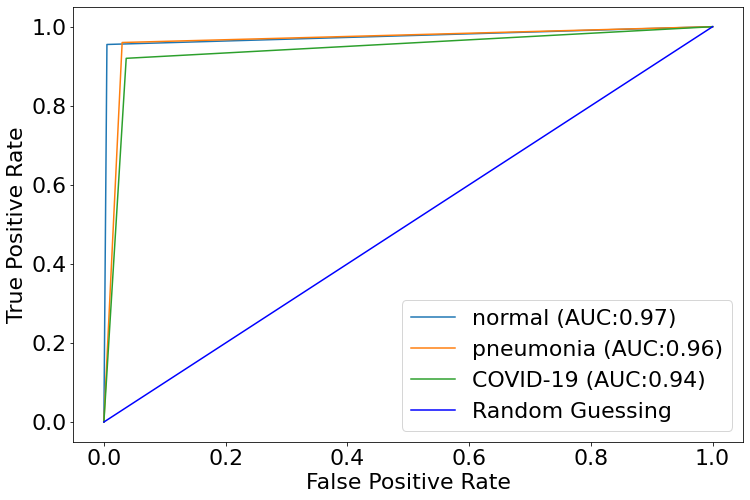
\includegraphics[width=\textwidth]{figures/au-roc-4.png}
         \caption{Fold 4}
         \label{fig:auroc-fold-4}
     \end{subfigure}
     
     \vspace{10mm} %10mm vertical space
     \begin{subfigure}[b]{0.49\textwidth}
         \centering
         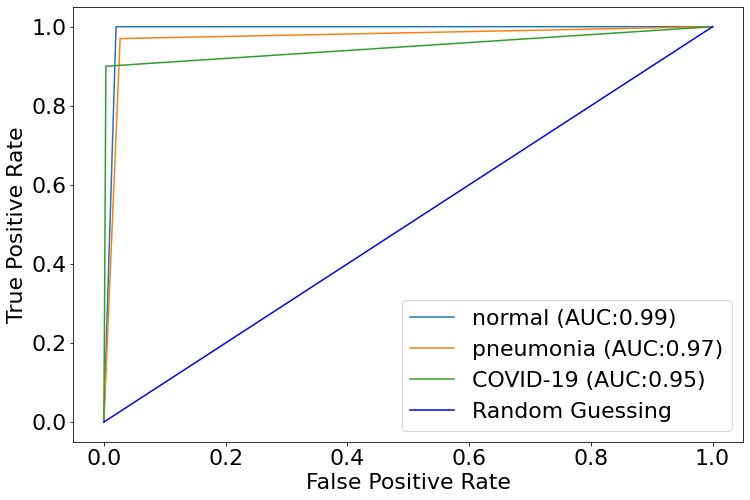
\includegraphics[width=\textwidth]{figures/au-roc-5.png}
         \caption{Fold 5}
         \label{fig:auroc-fold-5}
     \end{subfigure}
        \caption{AU-ROC graphs for the Xception model.}
        \label{fig:au-roc-all}
\end{figure}
\begin{landscape}
    \centering
    \vspace*{\fill}
    \begin{figure}[H]
        \centering
        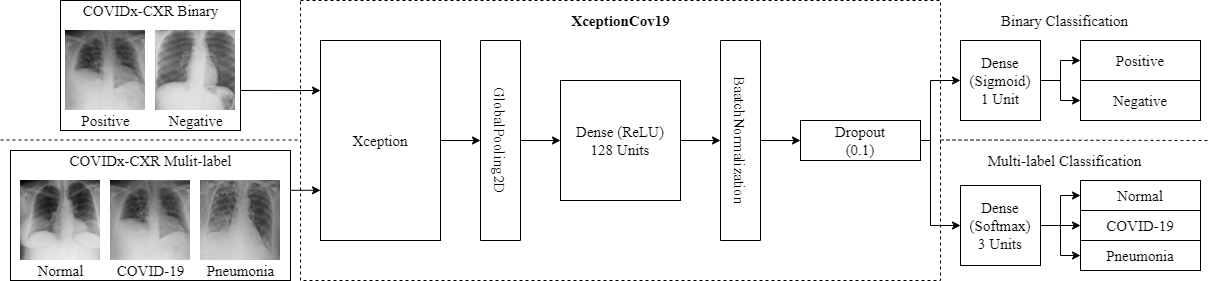
\includegraphics[width=1.5\textwidth]{figures/xceptioncov19.png}
        \caption{The final XceptionCov19 model.}
        \label{fig:xceptioncov19}
    \end{figure}
    \vfill
\end{landscape}